\section{Extended Reasoning Capability Boundary After RLVR}
\label{sec:benchmark_analysis}

In this section, we present concrete benchmark evaluations that demonstrate how RLVR can fundamentally enhance the reasoning abilities of LLMs. This enhancement goes beyond mere improvements in sampling efficiency; it also expands the reasoning capability boundary. However, to effectively observe this enhancement, it is crucial to adopt an appropriate RLVR training recipe, select challenging benchmarks that are free from data contamination, and utilize reliable evaluation metrics. Without these measures, one might only observe improvements in sampling efficiency, with no actual change in reasoning capacity. Below, we discuss two representative cases from both the math and code domains, showcasing genuinely extended reasoning boundaries.


\subsection{Math Reasoning}

\begin{figure}[t]
\begin{center}
%\framebox[4.0in]{$\;$}
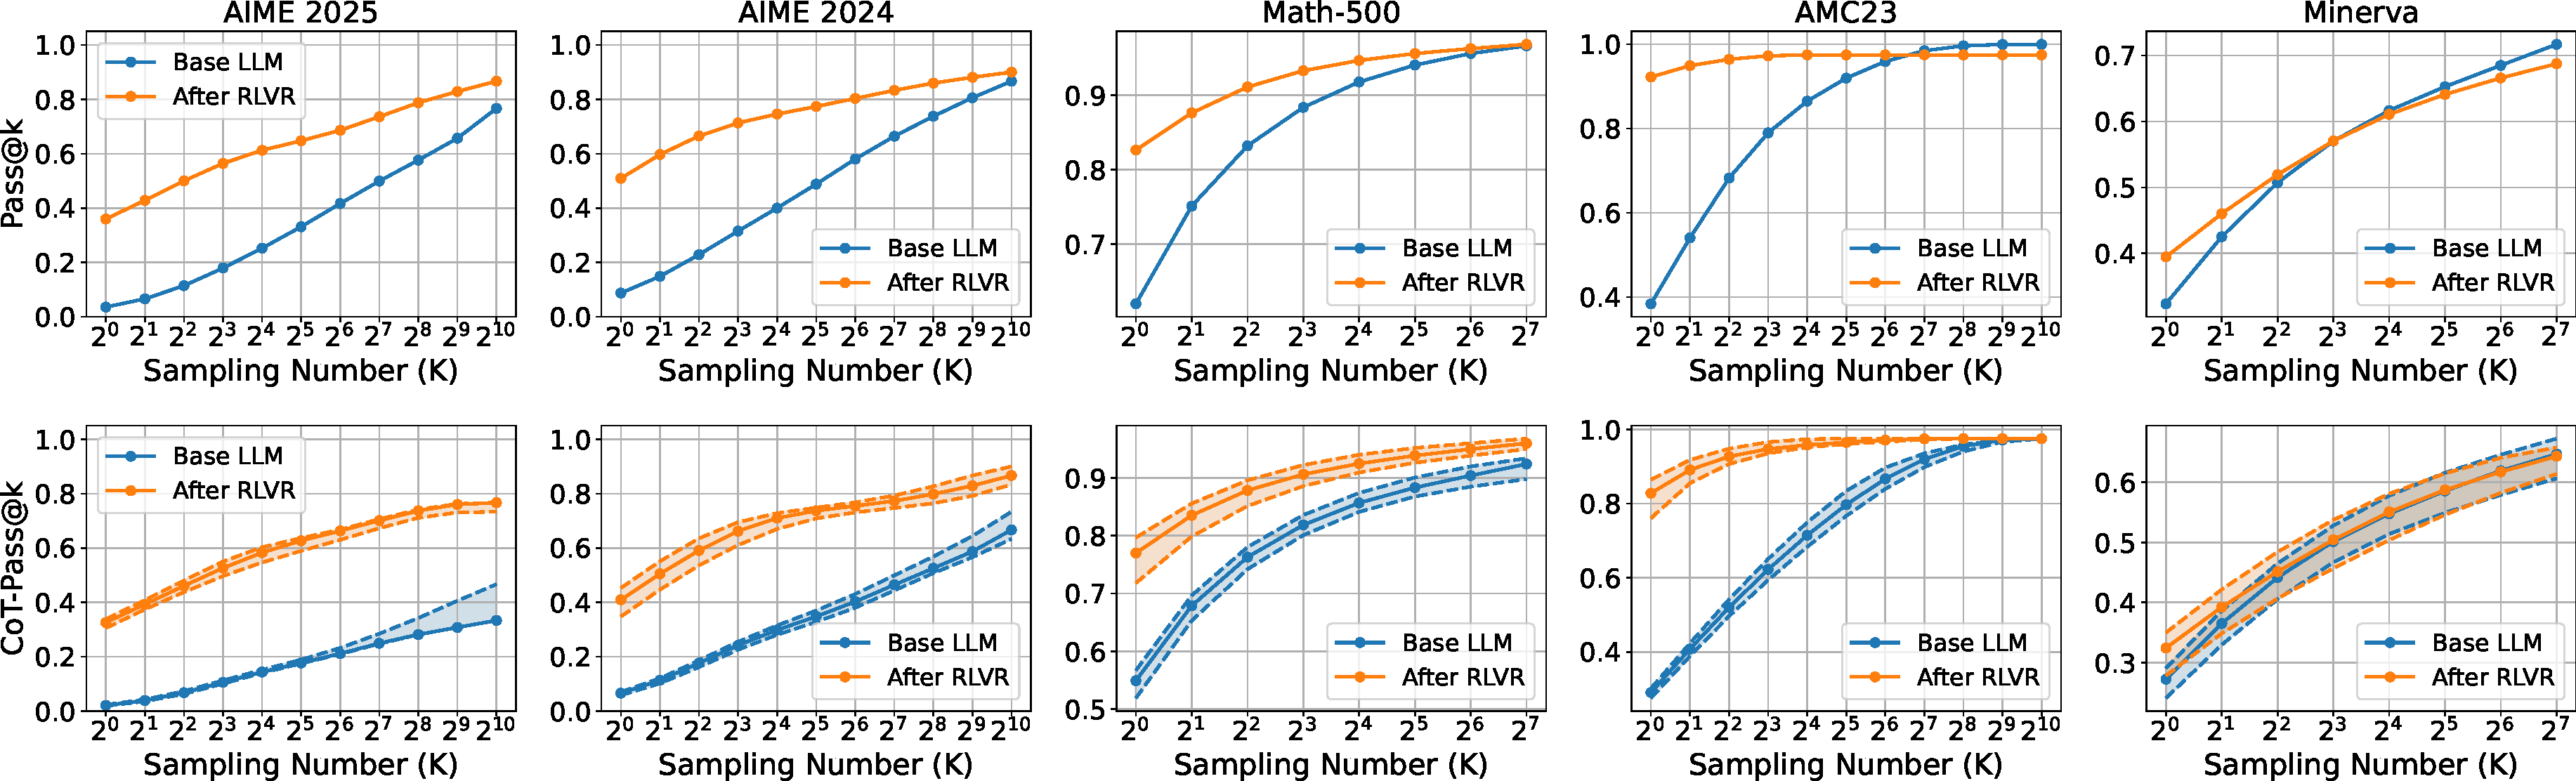
\includegraphics[width=1.0\textwidth]{figures/benchmark_cot_correct.pdf}
\end{center}
\caption{Comparisons of Pass@K (the top row) and CoT-Pass@K (the bottom row) on five math benchmarks (different columns) to show how RLVR could improve base LLMs. Here the base LLM is Qwen2.5-32B, and the post-RLVR model is DAPO-Qwen-32B. For CoT-Pass@K, we perform multiple verifications for each CoT using DeepSeek-R1-0528-Qwen3-8B, and display the results determined by \emph{any-correct}, \emph{all-correct}, and \emph{majority-correct} strategies, which constitute the shaded area in lower subplots.}
\label{fig:cot_passk_math_bench_dapo}
\end{figure}


We begin by revisiting the Pass@K experiments conducted on the open-source model, DAPO-Qwen-32B~\citep{yu2025DAPO-Zero}, which successfully reproduced R1-Zero~\citep{guo2025deepseek-r1} using the base LLM, Qwen2.5-32B~\citep{qwen2024Qwen2.5}, and a curated set of $17k$ mathematical problems. A key contribution of our work is the introduction of a novel evaluation metric, CoT-Pass@K, which emphasizes the importance of evaluating the correctness of detailed reasoning steps for mathematical questions, rather than relying solely on answer correctness.

However, precisely measuring the correctness of CoTs at scale is inherently challenging due to the unstructured, lengthy, and complex nature of math CoTs. Fortunately, we can leverage specialized open-source LLMs, such as DeepSeek-R1-0528-Qwen3-8B~\citep{deepseek2025R1-0528}, as a powerful yet lightweight verifier, employing an LLM-as-a-CoT-Judge paradigm. In this study, we use this verifier multiple times for each reasoning CoT generated by DAPO-Qwen-32B and Qwen2.5-32B, employing three distinct strategies to assess CoT correctness: \emph{any-correct} (at least one verification returns correct), \emph{all-correct} (all verifications must return correct), and \emph{majority-correct} (the majority vote determines the outcome). To further ensure the reliability of these verifications, we manually inspect cases where the Pass@K metric yields a small positive value, but the CoT-Pass@K metric returns zero.
The details of our LLM-as-a-CoT-Judge approach can be found in Appendix~\ref{supp_sec:verify_details}.

Figure~\ref{fig:cot_passk_math_bench_dapo} presents a comprehensive comparison using both Pass@K and CoT-Pass@K metrics across prominent math-reasoning benchmarks. As shown in the top row, the Pass@K results align with the observations in~\citep{yue2025RLVR_limit}: the performance of the base LLM quickly catches up with and even surpasses the post-RLVR model as $K$ increases. However, in stark contrast, the CoT-Pass@K results on AIME 2024 and AIME 2025 reveal a consistent and significant performance gap between the models across all values of $K$ (up to 1024). This gap is particularly pronounced on AIME 2025, possibly due to its complete absence of unintentional data contamination, as it was released after the base model’s training cutoff. We perform manual inspections to ensure the distinct gaps observed using the CoT-Pass@K metric are reliable (see examples in Appendix~\ref{supp_sec:aime24_case} and~\ref{supp_sec:aime25_case}). Our LLM verifier effectively identifies critical errors, which we agree should be rejected. These results demonstrate the extended reasoning boundary of DAPO-Qwen-32B over Qwen2.5-32B.

Additionally, we observe that on other benchmarks such as MATH-500 and AMC23, the effects of RLVR seem less pronounced, as the base LLM is already capable of solving these problems correctly with sufficient attempts. This may be due to 1) the problems being simple enough for the base LLM to solve using its existing knowledge, or 2) the problems being part of its pre-training data, allowing the base LLM to recall the correct solution after multiple trials. Distinguishing between these possibilities is challenging without knowing the exact training data used for Qwen2.5-32B. Furthermore, on the Minerva benchmark, the post-RLVR model shows no improvement, likely due to a train-test domain mismatch. Minerva contains numerous physics problems and free-form answers, while the DAPO training data was restricted to math problems with integer answers. These results do not undermine the effectiveness of RLVR; rather, they highlight the importance of selecting appropriate benchmarks for evaluating RLVR progress.

\subsection{Code Reasoning}

\begin{figure}[t]
\begin{center}
%\framebox[4.0in]{$\;$}
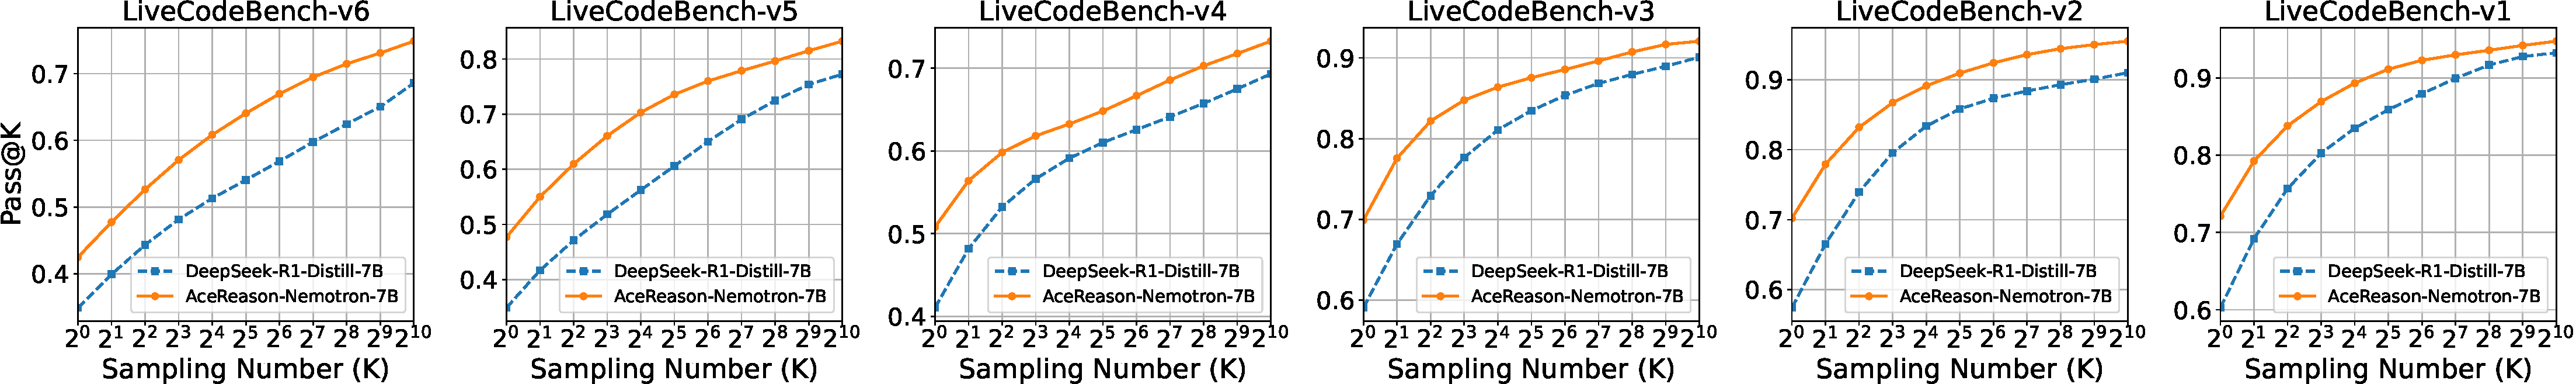
\includegraphics[width=1.0\textwidth]{figures/ysy_eval_ace_lcb_all.pdf}
\end{center}
\caption{Comparisons of Pass@K across six LiveCodeBench versions to show how much RLVR could enhance distilled LLMs. Here the distilled LLM is DeepSeek-R1-Distill-Qwen-7B, and the post-RLVR model is AceReason-Nemotron-7B.}
\label{fig:cot_passk_code_bench_ace}
\end{figure}


Unlike RLVR for mathematical problems, where the correctness of extracted answer tokens is used as a proxy for passing, code reasoning relies on the actual execution of generated code snippets to verify correctness, significantly reducing the likelihood of guessing. Therefore, Pass@K serves as a reliable evaluation metric for code reasoning tasks.

In this section, we reproduce the Pass@K experiments across different versions of LiveCodeBench~\citep{Jain2025LiveCodeBench} to compare the performance of AceReason-Nemotron-7B~\citep{chen2025AceReason-Nemotron} with its pre-RLVR counterpart, DeepSeek-R1-Distill-Qwen-7B~\citep{guo2025deepseek-r1}. As shown in Figure~\ref{fig:cot_passk_code_bench_ace}, we observe that AceReason-Nemotron-7B exhibits clear Pass@K improvements over DeepSeek-R1-Distill-Qwen-7B on most benchmark versions, even though the latter is a distillation model already demonstrating remarkable reasoning capabilities. These results suggest that even for distillation models, a high-quality RLVR training recipe can significantly extend the reasoning capability boundary, particularly for competitive coding tasks.

To further confirm the success of RLVR in extending reasoning boundaries for coding tasks, we evaluate another post-RLVR model, Skywork-OR1~\citep{he2025Skywork-OR1}, which has a fully reproducible training recipe publicly available. Detailed results on LiveCodeBench-v6 can be found in Appendix~\ref{supp_sec:benchmark_skywork_or1}, where we observe a consistent Pass@K gap between Skywork-OR1 and DeepSeek-R1-Distill-Qwen-7B. Specifically, we find that only medium and hard problems in LiveCodeBench-v6 contribute to the differentiation between these two models for large $K$ values, underscoring the importance of selecting challenging benchmarks.



